\section{Autocorrelation Structure of Forecast Errors (Q4, Q5)}

\subsection{Average ACF and PACF Behavior}

We created box plots of the averaged autocorrelation function (ACF) and the partial autocorrelation function (PACF) for the raw forecast errors of all eight variables. The plots are based on lead time for each forecast run across all 896 sites and all three years. Each sequence represents a 48-hour forecast run at one site, and the lags in the graphs represent the differences between lead times.

The main findings are as follows.
\begin{itemize}
    \item From the ACF graphs, GHI errors remain related for about 3 lags, temperature for about 6 lags, pressure for about 9 lags, and RH for about 6 lags.
    \item In the PACF plots, the first lag is clearly dominant for all variables. The strongest PACF lag-1 value was for temperature, with an average value of about 0.88, while the weakest was for wind direction, with an average value of about 0.27.
    \item U10, V10, wind speed, and wind direction seem to have similar behavior. They remain related for around 5 hours, then the autocorrelation centers around zero for the remaining lags.
\end{itemize}

\begin{figure}[H]
    \centering
    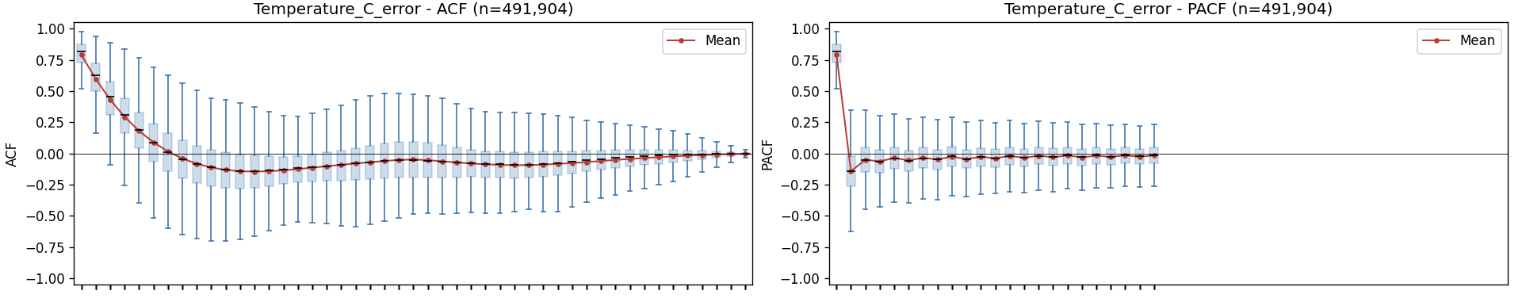
\includegraphics[width=\textwidth]{figures/Q4 & Q5/Temperature_ACF_PACF.png}
    \caption{ACF vs. lag on the left and PACF vs. lag on the right for temperature. The ACF values drop quickly from lag 1 onward. By around lags 8--15, most variables are close to zero or slightly negative.}
    \label{fig:Temperature_ACF_PACF}
\end{figure}

\begin{figure}[H]
    \centering
    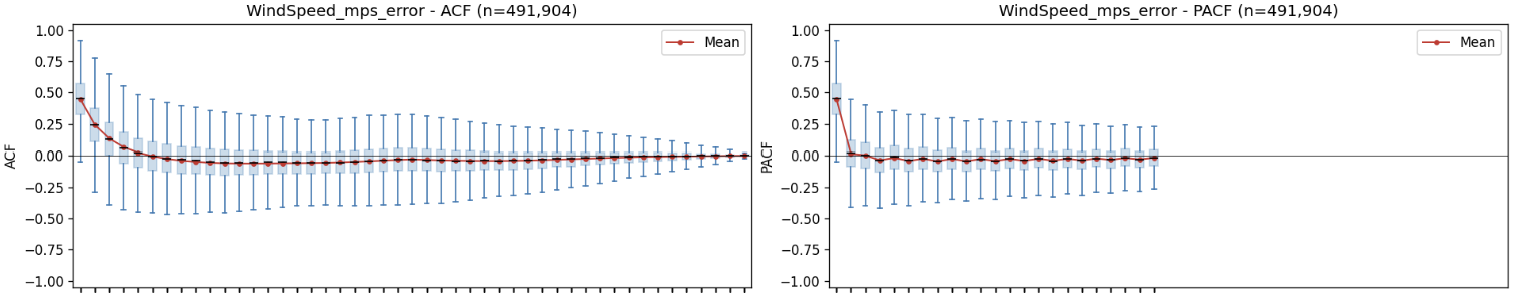
\includegraphics[width=\textwidth]{figures/Q4 & Q5/WindSpeed_ACF_PACF.png}
    \caption{ACF vs. lag on the left and PACF vs. lag on the right for wind speed.}
    \label{fig:WindSpeed_ACF_PACF}
\end{figure}

\subsection{Differences by Season, Year, Zone, and Time of Day}

We calculated the average ACF and PACF values for sequences grouped by four seasons, three years, four times of day, and nine zones. After that, we ran the Kruskal-Wallis test to see whether the average ACF and PACF curves differed by season, year, time of day, and zone, as shown in Figure~\ref{fig:kw_heatmap}.

The main findings are as follows.
\begin{itemize}
    \item The strongest difference appears in pressure ACF by season with $p = 0.12$, but this is still not below the usual 0.05 significance level.
    \item Wind variables show some weaker differences by season, such as U10 and V10 with $p = 0.19$, and wind speed with $p = 0.20$.
\end{itemize}

\begin{figure}[H]
    \centering
    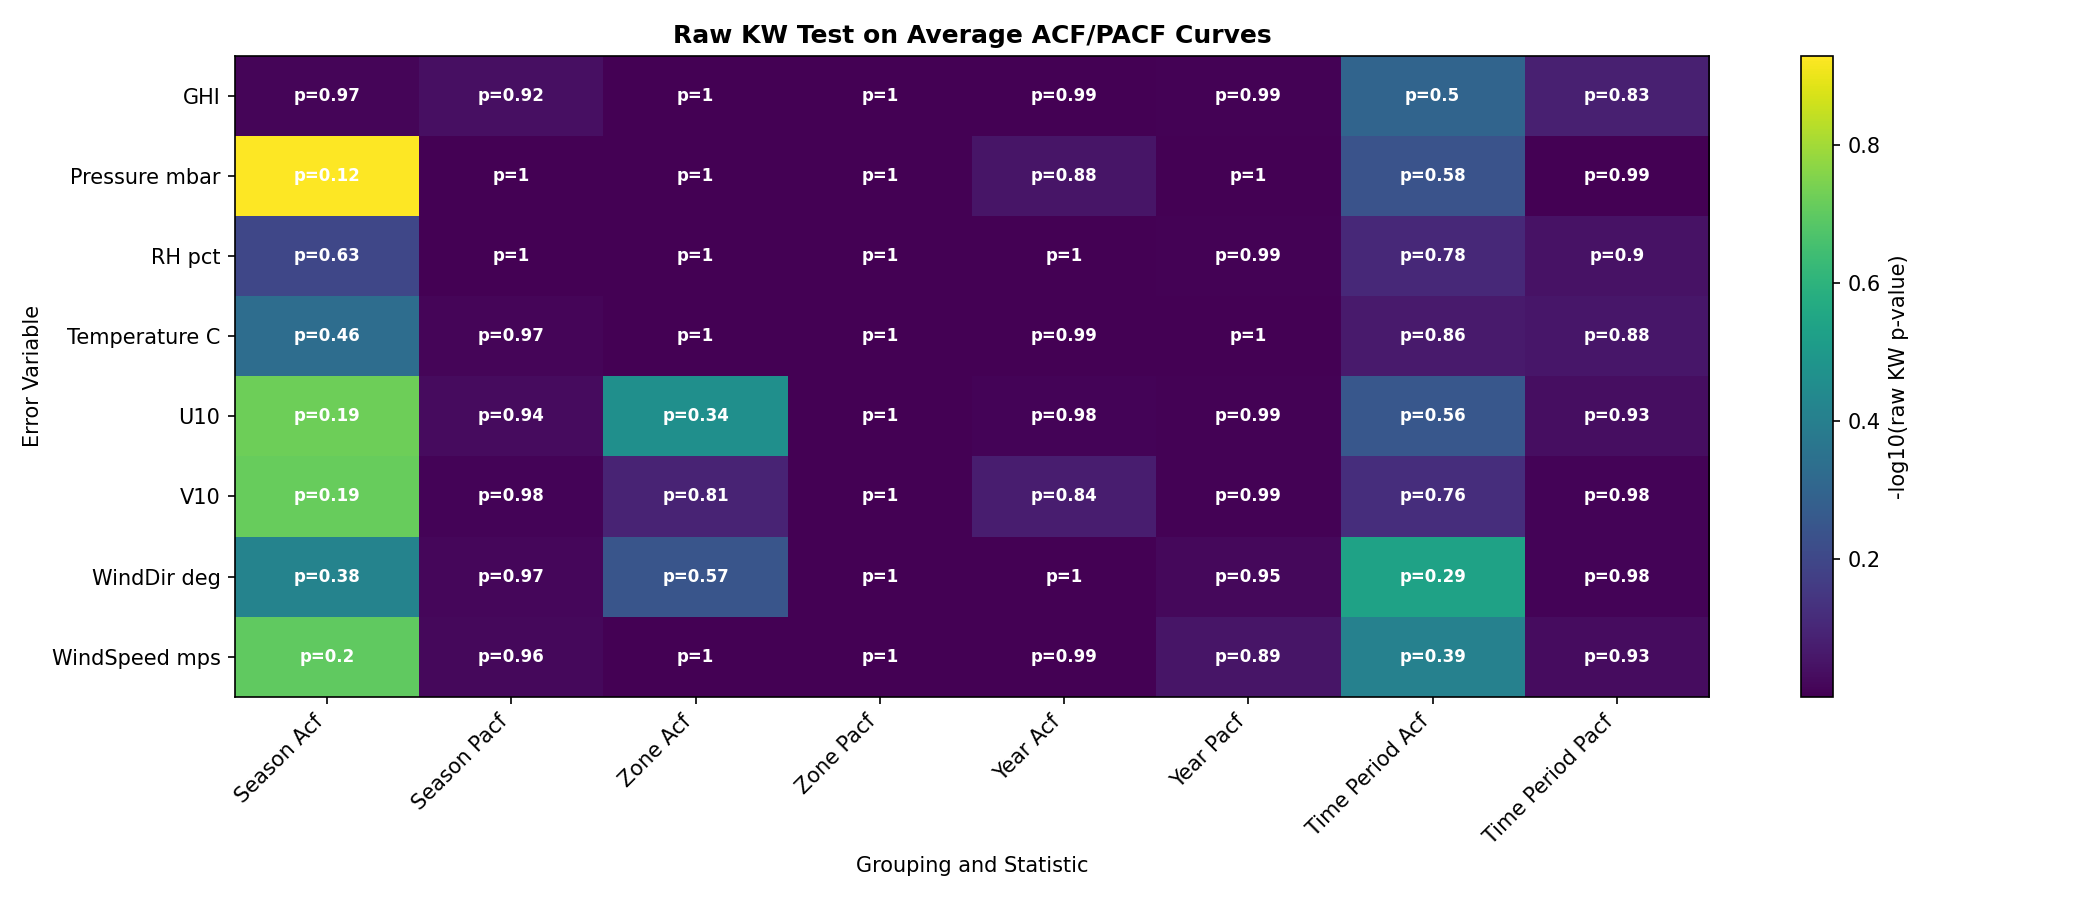
\includegraphics[width=\textwidth]{figures/Q4 & Q5/acf_pacf_average_curve_raw_kw_heatmap.png}
    \caption{The rows list the error variables, and the columns show the grouping being compared: season, zone, year, or time of day, separately for ACF and PACF. Each cell shows the raw Kruskal-Wallis p-value, where smaller p-values suggest stronger differences between the average curves.}
    \label{fig:kw_heatmap}
\end{figure}

\subsection{Implications}

Forecast errors show short-term persistence. However, this persistence weakens as the gap between forecast hours increases. If the model has an error at one forecast hour, nearby forecast hours tend to have similar errors. Most of the direct autocorrelation structure appears at the immediately previous forecast hour. Moreover, there is no strong statistical evidence that the correlations differ meaningfully across years and zones. Season and time of day show slightly more variation than zone and year, but the differences are still not statistically significant.
